\documentclass[14pt]{extarticle}
\usepackage{amsmath}
\usepackage{amssymb}
%\usepackage{tikz}
%\usetikzlibrary{calc}
%\usetikzlibrary{trees}
\usepackage{hyperref}
\usepackage{graphicx}
\graphicspath{ {../../chap11/} }
\usepackage[top=0.75in, bottom=0.75in, left=0.75in, right=0.75in]{geometry}
%\newcommand*{\Scale}[2][4]{\scalebox{#1}{\ensuremath{#2}}}%
\usepackage[shortlabels]{enumitem}
\usepackage[most]{tcolorbox}
\definecolor{bg}{RGB}{255,249,227}
% \usepackage{showframe}

\title{\vspace{-5ex}Math 208 Section 11.1}
\date{\vspace{-10ex}}
\usepackage{multicol}
\setlength{\columnsep}{1cm}
\setlength{\parindent}{0pt}
\usepackage{parskip}
\setlength{\parskip}{10pt} % 1ex plus 0.5ex minus 0.2ex}
%\usepackage{ragged2e}



\begin{document}
	\maketitle
	
\section{Homework, Reading, and Other}
\begin{itemize}
	\item Section 10.7
	\item Section 11.1
\end{itemize}

\section{Goals}
\begin{itemize}
	\item Understand what the first derivative tells us about the graph of a function
	\item Create and interpret a sign chart
	\item Draw a graph using the sign chart
\end{itemize}


\section{Section 11.1: First Derivative and Graphs}
\subsection{Preliminaries}
Let's first take a look at \textit{sign charts}. What is a sign chart?
\begin{tcolorbox}[enhanced jigsaw,colback=bg,boxrule=0pt,arc=0pt]
	A \textbf{Sign Chart} uses a formatted table to indicate whether a function takes a negative or positive value in an interval.
	\\\\
	Steps to create a sign chart, given a function $f(x)$:
	\begin{enumerate}
		\item Find all values of $x$ where $f(x)=0$ or $f(x)$ is discontinuous i.e. the denominator $=0$.
		\item Plot the numbers from step 1 on a number line.
		\item Select a test number, $(t)$, in each interval from step 2. Determine the whether $f(t)$ is negative or positive.
		\item If the test was positive, place a \textbf{+} in that interval. If the test was negative, place a \textbf{-} in that interval.
	\end{enumerate}
	\vspace{1em}
	\textbf{Partition numbers} are the name for the values of x where $f(x)=0$ or $f(x)$ is discontinuous.
\end{tcolorbox}

\subsubsection{Examples}
\textbf{Ex1}
Create a sign chart for $f(x)= 2x-4$. $$f(x) = 0 \text{ at } x=2$$
Let's try the test points $t_1=0$ and $t_2=4$.
\begin{align*}
	f(0) &= -4 \\
	f(4) &= 4
\end{align*}
From this we create our sign chart of
\begin{verbatim}
 x   |      2      
f(x) | ---  0  +++
\end{verbatim}

That should give you an idea of how to create and use a simple sign chart. We'll see more examples as we work through this chapter.


\subsection{Increasing and Decreasing}
Consider the graph of $f(x)=x^2-3x$.

\begin{center}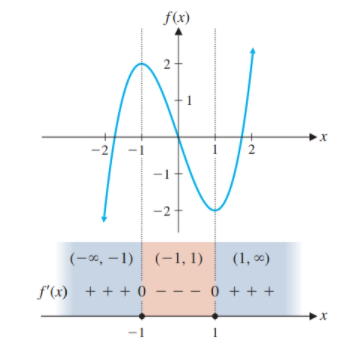
\includegraphics[width=0.55\linewidth]{11-1-a1}\end{center}

By examining the graph, we determine that $f(x)$ is increasing on the interval $(-\infty, -1)$, decreasing on the interval $(-1,1)$, and increasing on the interval $(1, \infty)$. We also note that \textit{increasing} means that the slope is positive, while \textit{decreasing} means that the slope is negative.

The slope of the tangent line at a given point is equal to the \textbf{derivative of} $\mathbf{f(x)}$.

\subsection{Understanding the graph and derivative}
Local minima and maxima occur when the slope of the tangent line is horizontal, i.e when $f'(c) = 0$. But having $f'=0$ is not sufficient to say that we have found a local minima or maxima. The function, $f$, must pass also from
\begin{itemize}
	\item increasing to decreasing ($f'+++$ to $f'---$) for a \textbf{maximum}
	\item decreasing to increasing ($f'---$ to $f'+++$) for a \textbf{minimum}
\end{itemize}
\begin{center}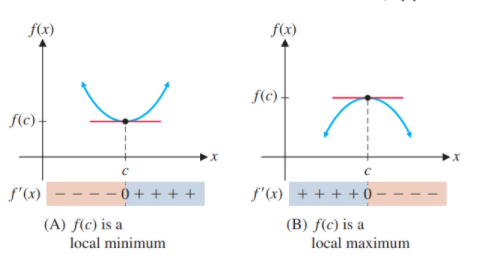
\includegraphics[width=0.7\linewidth]{11-1-a2}\end{center}
\begin{center}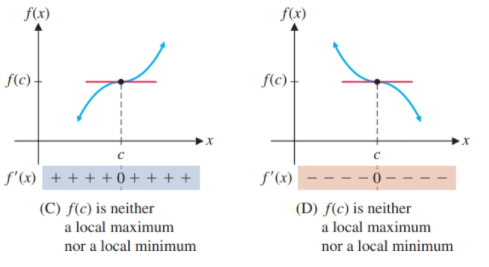
\includegraphics[width=0.7\linewidth]{11-1-a3}\end{center}
\vspace{1em}
And sometimes when f'(c) is not defined. $f'$ is not defined when the slope is infinite or the function is not "smooth".
\begin{center}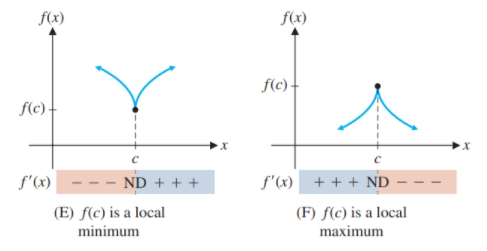
\includegraphics[width=0.7\linewidth]{11-1-a4}\end{center}
\begin{center}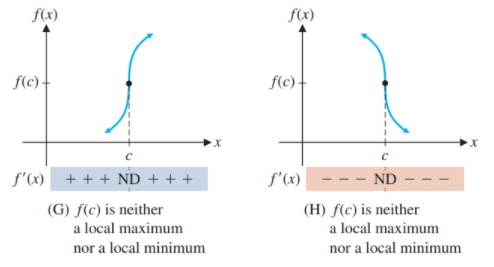
\includegraphics[width=0.7\linewidth]{11-1-a5}\end{center}
\vspace{1em}
Notice the colored bars under the graphs. These \textbf{sign charts} indicate the behavior of $f'$ in those intervals of the graph.

\subsection{Partition Numbers and Critical Numbers}
\begin{itemize}
	\item Recall that partition numbers are the values of x where $f(x)=0$ or $f(x)$ is discontinuous.
	\item Critical numbers are just the partition numbers of $f'$. Meaning, the values of x where $f'(x)=0$ or $f'(x)$ is discontinuous.
\end{itemize}

\cleardoublepage

\subsection{Examples}
\textbf{Ex2}
Find the critical and partition numbers of f, the intervals on which f is increasing, and those on which f is decreasing, for $f(x) = 1 - x^3$.

\begin{multicols}{2}
\begin{align*}
	f(x) &= 0 \text{ when } x=1 \\
	& \text{Test points } x = 0, x=2 \\
	&f(0)= 1, f(2) = -1 \\\\
	f'(x) &= -3x^2 = 0 \text{ when } x=0 \\
	& \text{Test points } x =-1, x=1 \\
	&f'(-1)= -3, f'(1) = -3
\end{align*}
\vspace{2em}
\begin{verbatim}
x   |      0      1
f(x)  | +++  1  +++ 0 ---
f'(x) | ---  0  ---   ---
\end{verbatim}
\vfill\null
\columnbreak 
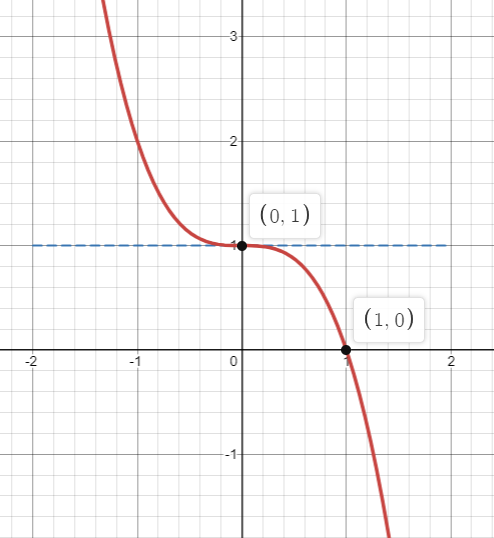
\includegraphics[width=1\linewidth]{11-1-a6}
\end{multicols}

\vspace{2em}

\textbf{Ex3}
Make a sign chart for $f(x) = (1-x)^{1/3}$.	
\begin{multicols}{2}
	\begin{align*}
		f(x) &= 0 \text{ when } x=1 \\
		& \text{Test points } x = 0, x=2 \\
		&f(0)= 1, f(2) = -1 \\
		f'(x) &= -(1/3)(1-x)^{-2/3} = 0 \text{ Never}\\
		 &\text{But is undefined when } x=1 \\
		& \text{Test points } x =0, x=2 \\
		&f'(0)= -1/3, f'(2) = -1/3
	\end{align*}
\begin{verbatim}
  x   |      1
f(x)  | +++  0  ---
f'(x) | ---  ND ---
\end{verbatim}
	\vfill\null
	\columnbreak 
	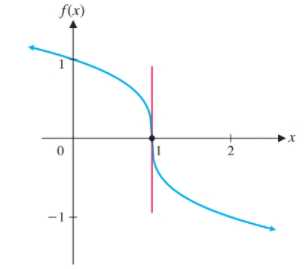
\includegraphics[width=1\linewidth]{11-1-a7}
\end{multicols}

\textbf{Ex4}
Make a sign chart for $f(x) = \frac{1}{x-2}$.	
\begin{multicols}{2}
	\begin{align*}
		f(x) &= 0 \text{ Never. But ND at } x=2 \\
		& \text{Test points } x =1, x=3 \\
		&f(1)= -1, f(3) = 1 \\
		f'(x) &= -(x-2)^{-2} = 0 \text{ Never}\\
		&\text{But is undefined when } x=2 \\
		& \text{Test points } x =1, x=3 \\
		&f'(0)= -1, f'(2) = -1
	\end{align*}
\begin{verbatim}
  x   |      2
f(x)  | --- ND +++
f'(x) | --- ND ---
\end{verbatim}
	\vfill\null
	\columnbreak 
	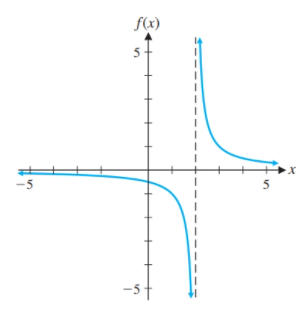
\includegraphics[width=1\linewidth]{11-1-a8}
\end{multicols}

\textbf{Ex5}
\begin{center}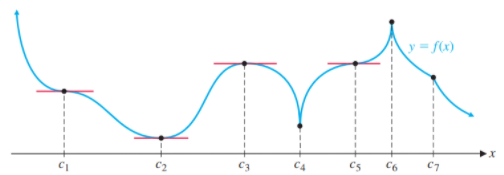
\includegraphics[width=1\linewidth]{11-1-3}\end{center}
\vspace{1em}
For the graph above, do the following: Construct a sign chart and Identify local maxima and minima. (similar to problems 9-17)
\begin{verbatim}
  x   |      c1      c2      c3      c4      c5      c6      c7
f'(x) | ---  0  ---  0  +++  0  ---  ND +++  0  +++  ND ---  ND ---
\end{verbatim}
\noindent\rule{\textwidth}{1pt}
\begin{verbatim}
f(x)  | +++ Ifl +++ Min +++ Max +++ Min +++ Ifl +++ Max +++ Ifl +++
\end{verbatim}
\vspace{1em}

\textbf{Ex6} (35) Create and interpret the sign chart for $f(x) = -2x^2 -16x -25$. Then graph the function,

When does $f(x) = 0$? Use the quadratic equation.
\begin{align*}
	\sqrt{b^2 -4ac} &= 7.48 \\
	&x_1 = -5.871, x_2=-2.129 \\
	& \text{Test points } x =-10, x=-4, x=0 \\
	&f(-10)= -65, f(-4) = 7, f(0)=-25 \\\\
\end{align*}
When does $f'(x) =0$?
\begin{align*}
	f'(x) &= -4x-16 =0 \text{ at } x=-4\\
	& \text{Test points } x =-5, x=0 \\
	&f'(-5)= 4, f'(0) = -16 \\\\
	f(4) &= -121
\end{align*}

\begin{verbatim}
  x   |     -5.8     -4      -2.1
f(x)  | ---    0 +++  7  +++    0 ---
f'(x) |          +++  0  ---         
\end{verbatim}

Therefore $f(-4)=7$ is a maximum. Now graph the function.

\begin{tcolorbox}[enhanced jigsaw,colback=bg,boxrule=0pt,arc=0pt]
	\textbf{Intercepts and Local Extrema of Polynomials}
	
	If $f(x)$ is a polynomial function of degree $n\geq 1$, then $f$ has at most $n$ x-intercepts and at most $n-1$ local extrema.
\end{tcolorbox}

\textbf{Ex6} (43) Create and interpret the sign chart for $f(x) = x^4 +4x^3 +30$. Then graph the function.

Start with a consideration of this function. We know that there are at most 4 x-intercepts and at most 3 local extrema. Let's try to find the zeroes of the function.
\begin{align*}
	f(x) &=0 = x^4 +4x^3 +30 \\
	&x^4 +4x^3 = -30\\
	&x +4 = -\frac{30}{x^3}
\end{align*}
Notice: In order for the left hand side (LHS) to be negative, $x< -4$. But when $x$ is negative, the RHS is positive. The only possible interval is $(-4, 0) $. We'll comeback to this but let's now evaluate $f'$.

\begin{align*}
	f'(x)&=4x^3 + 12x^2  &\tag{When does f' equal 0?}\\
	0 &= 4x^2(x + 3) \\
	x &= -3 &\tag{Root} \\
	x &= 0 &\tag{Double root} \\\\
	\text{Test points } x &=-10, x=-1, x=1 \\
	f'(-10) &= -4000 + 1200 < 0 \\
	f'(-1) &= -4 + 12 > 0 \\
	f'(1) &= 4 + 12 > 0 \\\\
	f(-3) &= 3 \\
	f(0) &= 30 \\
	f(-10) &= 6030 > 0 \\
	f(-1) &= 27 > 0 \\
	f(1) &= 35 > 0
\end{align*}
\begin{verbatim}
  x   |     -3        0      
f(x)  | +++  3  +++  30 +++ 
f'(x) | ---  0  +++   0 +++  
            Min     Ifl
\end{verbatim}
$f(x)$ has a minimum at $x=-3$ and an inflection point at $x=0$. Since $f$ is always positive, the function has no zeros. Now graph the function.


\noindent\rule{\textwidth}{1pt}
{\footnotesize Copyright (C) 2021 Garold Dalton --- Released under GNU General Public License v3.0}


\cleardoublepage	
	
\end{document}
